% !TEX root = ../main.tex
\section{Related Work}
\label{sec:related}
\begin{figure}
\centering
\subfloat[ARToolkit]{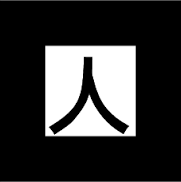
\includegraphics[width=50px, height=50px]{figs/tags/artoolkit}} \quad
\subfloat[ARTag]{
\includegraphics[width=50px, height=50px]{figs/tags/artags}} \quad 
\subfloat[AprilTag]{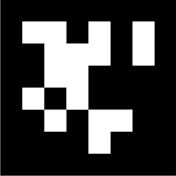
\includegraphics[width=50px, height=50px]{figs/tags/apriltags}} \\
\subfloat[RUNE-Tag]{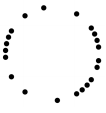
\includegraphics[width=50px, height=50px]{figs/tags/rune}} \quad
\subfloat[Intersense]{
\includegraphics[width=50px, height=50px]{figs/tags/intersense}}
\caption{Different types of popular fiducial tags. ARToolkit, ARTags, and AprilTags are square tags with black borders. RUNE-tags and Intersense use different circle features as landmarks}
\label{fig:exp_setup}
\end{figure}
	Be able to obtain highly accurate pose estimation has been an important research area in robotics. There are numerous algorithms developed that rely only on RGB or grey scale images. Most of these methods rely on solving the projection geometry of some detected features and then minimize the reprojection error of the features in the image space [].  Similarly, methods such as Iterative Closet Point were developed to solve the pose estimation problem using range data by minimizing the Euclidean distance between the model and the depth data. Recently, there are some approaches proposed to enhance the accuracy of traditional algorithms by fusing RGB and depth data in various problems by using extended Kalman filter []. Compared to the single sensor approaches, algorithms utilizing RGBD data are more accurate and performs well in noisy situations where other approaches fail. 
	
	Using fiducial marker is an example of pose estimation methods exploiting easily detectable features in the RGB space. Although there is an abundance of unique tag designs. most of them carry easily recognizable yet precise binary patterns in the inner region to encode information with. There are two large type of common tags: square tags and circle tags. 
	
	Circular tags are created to encode the payload using small circle patterns arranged in various shapes. The example of circular tags include Intersense[] and Rune tags[]. The perspective transformation of a circle is an ellipse, which can be used to directly compute the pose using back projection methods. The detection of circular features are generally more accurate to localize and thus generates better pose estimations at the cost of higher computation time. However, small circular features become hard to detect when they are far away from the camera or prospectively rotated and thus their effective range is much smaller than that of square tags. This characteristic making them less useful in applications with size constraints. 
	
	ARTags[], ARToolkit[], AprilTag[] and AprilTag 2[] are examples of squared based fiducial tags. The perspective projection of a square becomes a general quadrilateral which can be computed easily using any contour tracing algorithm. Given the scale of a single marker, the full 6-DOF pose can then be estimated using the corners of the quadrilateral. However, since they are detected using rectangles and lines, the accuracy of their corner point sub-pixel locations are limited. Among the square tags, ARToolkit is one of the earliest detection system and it was mainly used for Augmented reality applications. Instead of using a binary payload, it used various symbols to encode the tag and it was computationally expensive to decode the tag. Built on top of ARToolkit, ARTags and Apriltag reduced the computation time by using a 2D binary pattern as the payload. Both systems use the image gradient to compute the tag border making it robust to lighting changes and partial occlusions. Relative to the ARTags, Apriltag has a lower false positive rate as it uses a lexicode-based system that is invariant to rotation. In addition, the Apriltags have higher detection rates at further distances and at more difficult viewing angles. Recently AprilTag 2, improved upon the origin Apriltag, implemented a new boundary segmentation algorithm which further reduced the computing time for detection and increased the detection rate. Compared to circular tags, the advantages of the square tags are that they can be located very efficiently and they have reliable decoding schemes. Therefore, even though the square tags have slightly lower localization accuracy, they are more suitable for robotic applications that require a robust system.